\documentclass[11pt]{article}
\usepackage{graphicx}
\usepackage{fullpage}
\usepackage{fourier}
\usepackage{xspace}
\usepackage{booktabs}
\usepackage{wrapfig}

\title{cse13s asgn7 WRITEUP.pdf}
\author{Lucas Lee; CruzID: luclee}
\date{3/11/2022}
\begin{document}\maketitle

\section{Program Details}\label{ss:details}
This program will use Hash tables, Bloom Filters, and Bitvectors to find k most likely authors to a given text.

\section{Program issues}\label{ss:issues}
My program produces the same order of authors as the example binary when I run the program with the normal database, but it runs very slowly compared to the example. This is because my program uses an insertion method rather than the heap method which makes my program run at O(n). Other than this, my program's excessively long run time could be because I may be performing extra hash table lookups throughout the process of computing the distances between the texts and/or computing the Texts. \\
\\
In terms of the smaller databases, the program still runs a bit slow, but the difference is much less than the example binary. For the large databases, it takes about 3 minutes and a half, while running it on the small database is about 20 seconds to run. The accuracy on smaller text files is a bit off, but the order is generally correct with the larger database. There are some files in the small database that sometimes display the wrong ordering, but the only thing that it changes is that it swaps two different texts. The distances for these texts may have something to do with my lookup function, as when I would change the function for testing purposes, it would change the distance to be closer between those two texts. I believe this is when you run the small database to display 10 matches, and the two swapped authors are Henry James and H. G. Wells. Otherwise I have not seen any differences with the result ordering for my program and the example binary.
\section{Results when changing noise words}\label{ss:noise}
When changing the noise limit, the speed at which the identify binary changes, as well as many of the results.\\
If you increase the noise limit to around 200, meaning you filter out double the amount of words, the program runs a bit faster than it did before but not by a large difference. In the small database it makes it run a fraction of a second faster because it does not have to check the texts for as many words. For the default database, it decreases the run time by a couple seconds due to the text having much less words since there are much more texts to be created. \\

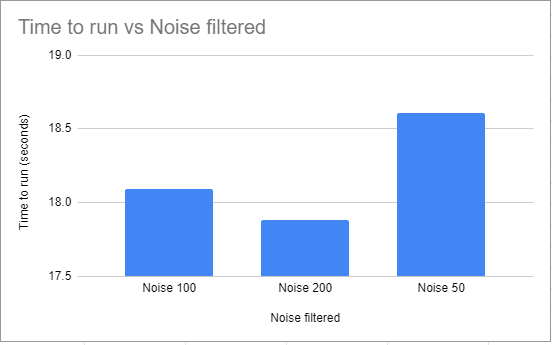
\includegraphics[width = 0.75\textwidth]{Graphs/Noise.PNG}

If you decrease the noise limit to about 50, you are leaving in half as many words that would normally be filtered out, making the program run slower. For the smaller database, this does not matter as much, most likely because the texts in the smaller database use the 50 words, that are not filtering out, very rarely. The run time changes for the small database by about half a second, while for the larger database, it runs for about an extra 15 seconds. 

\section{Comparing large vs small texts}\label{ss:size}
My program correctly is able to identify the closest authors using small texts. For extremely large texts, the amount of words is so large that the numbers calculated for the distances are very close. The distance values are sometimes extremely close when comparing two different large texts because of the amount of words in those texts.

\section{Comparing the different metrics}\label{ss:metrics}
In my program, all three of the metrics correctly generate the exact author, if given an author that exists in that database. Otherwise, my program, for the most part (in program issues) mimics the output from the example binary for each metric.

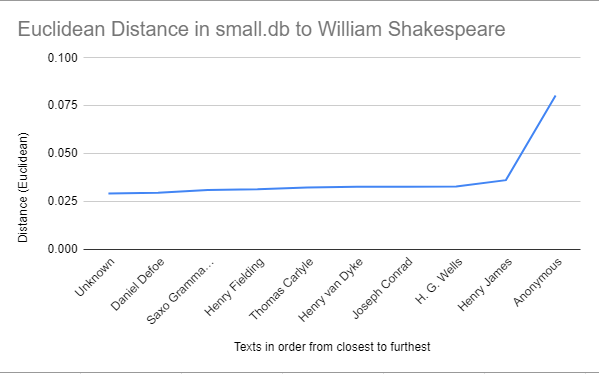
\includegraphics[width = 0.75\textwidth]{Graphs/Euclidean.PNG}

In the above graph is the nearest neighbors in small.db using the Euclidean distance from William Shakespeare's text, which matches the order of the example binary. While the Euclidean distance says that Saxo Grammaticus is the most likely author out of the small.db authors to be the one to write William Shakespeare's text, the other metrics don't agree.

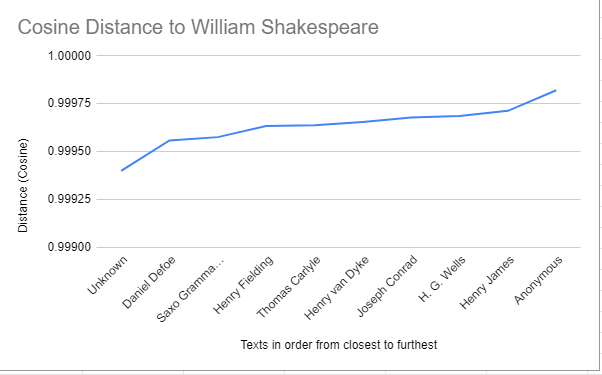
\includegraphics[width = 0.75\textwidth]{Graphs/Cosine.PNG}

The above graph shows the Cosine distance of the texts in small.db to William Shakespeare's text. The calculations essentially generate a larger sum based on the similarity of the texts and subtract that sum from 1. In the case for this calculation, the numbers are much higher than those of the Euclidean distance, and they also produce a different result. According to the Cosine distance calculation, the Unknown author is the most likely author to be the one to write Shakespeare's text.

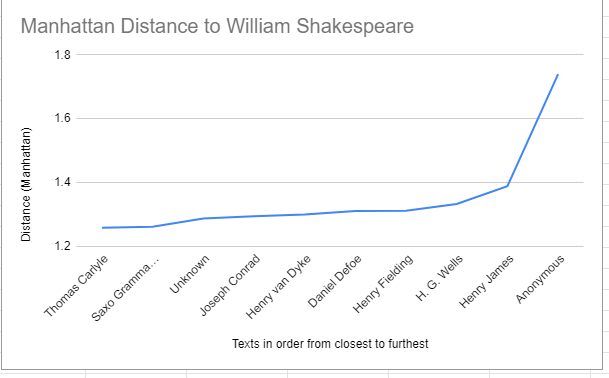
\includegraphics[width = 0.75\textwidth]{Graphs/Manhattan.PNG}

The above graph shows the Manhattan distance of the texts in small.db to Shakespeare's text once again. These calculations are even larger, since the calculation simply gets the sum of the difference between vectors. This metric claims that Thomas Carlyle is the most likely author of Shakespeare's text. All 3 of these metrics agree on which text is the most unlikely text, which is the anonymous text, but only Manhattan and Euclidean agree that the author is most likely either Thomas Carlyle or Saxo Gramaticus, since their values are extremely close in distance. Overall, all three of these distance calculations give different values and approximate the distance very differently. 

\section{Other Comments}\label{ss:comments}
This program took a long time to compile in Valgrind, even for the small database, so I did not check this program with the large database through Valgrind, but I would assume that if the program is able to run without memory leaks in the smaller database, that it would not cause a problem checking for leaks in a larger database. I also tried to decrease the floating point round off errors using long doubles instead of doubles, but since the specified return values for the given functions are in doubles, I was not able to decrease the rounding error by a lot.

\end{document}
